\documentclass[fleqn]{article}
\usepackage{amsmath}
\usepackage[dvips]{graphicx}
\bibliographystyle{plain}
%__________________________________
\begin{document}

\section*{\center Compression of an Elastic Billet}
\subsection*{\underline{Problem Description}}
This is an implementation of an example calculation from
\cite{guilkeyIMPM} in which an elastic billet is compressed by a
rigid platen.  See Section 5.1 of that manuscript for a complete description
of the problem.
 
\subsection*{\underline{Simulation Specifics}}
\begin{description} 
\item [Component used:] \hfill Implicit MPM
\item [Input file name:] \hfill billet.ups
\item [Command used to run input file:]\hfill sus billet.ups
\item [Simulation Domain:]\hfill    40.0 x 21.0 x 0.5 cm

\item [Cell Spacing:]\hfill \\ 
.5 x .5 x .5 cm

\item [Example Runtimes:] \hfill \\
 10 minutes   (1 processor, 3.0 GHz Xeon)\\

\item [Physical time simulated:] \hfill 0.2 seconds (50\% compression)

\item [Associate scirun network:] \hfill billet.srn

\end{description}

\section*{\underline{Results}}

Figure~\ref{figdisks} shows a snapshot of the simulation, at about
25\% compression of the billet.
\begin{figure}[b]
  \center
%  \scalebox{0.2}{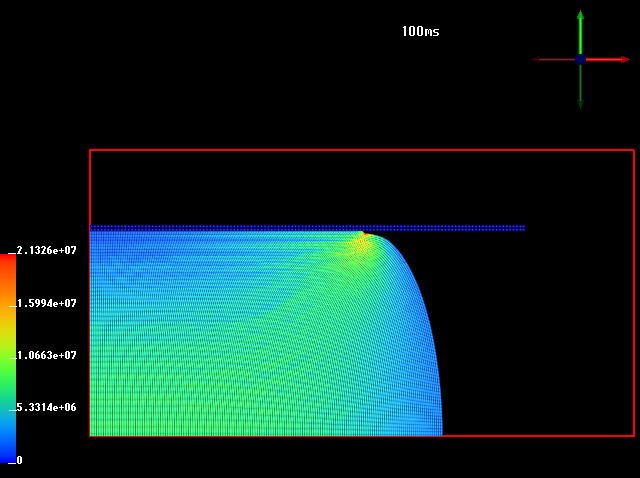
\includegraphics{billet.png}}
  \caption{Compression of an elastic billet.  Particles are
colored according to equivalent stress.}
  \label{figdisks}
\end{figure}

\bibliography{../references}

\end{document}
